\documentclass[oneside, 12pt]{article}
\usepackage[margin=1in]{geometry}
\usepackage{hyperref}
\usepackage{glossaries}
\usepackage{enumitem}
\usepackage{graphicx}
\usepackage{fancyhdr}
\usepackage{listings}
\usepackage{ntheorem}

\lstset{basicstyle=\small\ttfamily}
\setlength\parindent{0pt}

\title{Advanced Algorithms - Final project\\
       \vspace{3mm}\Large{Improve Ruby Hashing implementation using Tabulation}}
\author{Ana Maria Martinez Gomez - \texttt{\href{mailto:anamaria@martinezgomez.name}{anamaria@martinezgomez.name}}}
\date{\today}

\pagestyle{fancy}
\fancyhf{}
\lhead{Advanced Algorithms}
\rhead{Final project}
\lfoot{Ana Maria Martinez Gomez}
\rfoot{\thepage}

\renewcommand{\headrulewidth}{0.5pt}
\renewcommand{\footrulewidth}{0.5pt}

\makeglossaries
\newacronym{ror}{RoR}{Ruby on Rails}
\newacronym{mvc}{MVC}{Model-view-controller}
\newacronym{mri}{MRI}{Matz's Ruby Interpreter}

\theoremstyle{break}
\newtheorem{definition}{Definition}

\newcommand{\commitLinearShort}{11967eb}
\newcommand{\commitLinear}{11967ebf6e66d794d3efcb388b0e23cac045fc3e}
\newcommand{\commitQuadraticShort}{5a3fd57}
\newcommand{\commitQuadratic}{5a3fd57c3beeb86575cfeeb3d0dd458e5c016826}
\newcommand{\commitSimpleTabShort}{dbf917a}
\newcommand{\commitSimpleTab}{dbf917aa32f5e811da2d55c469580300aa430573}

\newcommand{\commitUrl}[2]{\href{https://github.com/Ana06/ruby/commit/#1}{#2}}

\begin{document}
\maketitle
\section{Introduction}

% Introduction about Ruby
Ruby is an interpreted, high-level, open source programming language, focused on simplicity and productivity.
It is mostly known because of \acrfull{ror}, a widely used \acrshort{mvc} web framework that powers companies like GitHub, Airbnb and Shopify. There are several implementations of Ruby.
The most popular one and the one we normally refer to when we speak about Ruby is \acrshort{mri}, the original Ruby interpreter written in C.
This is the one I will focus on for the project.\\


% Ruby hashing details
In Ruby, everything is an object and any object can be used as key or value in a hash.
We can create a hash with integers, strings, booleans, arrays or even hashes as keys:

\begin{lstlisting}
{ "str" => 0, true => 0, [1, 2, 3] => 0, { 2 => 1} => 0 }
\end{lstlisting}

In most cases, objects are converted to pseudorandom integers by using Murmur Hashing, accessible and overridable via the \lstinline{hash} method (a different seed is used for every session).\\

The original hashing algorithm used in Ruby was based on the one written in the late 1980's by Peter Moore at UC Berkeley.
The bucket in which an element was stored was determined by \lstinline{hash(key_object) % p}, where \lstinline{p} is a prime number close to a power of 2.
A linked list per bucket was used for collisions.
When any bucket had more than 5 elements, \lstinline{p} was increased and the values re-hashed.
Three years ago, \href{https://github.com/vnmakarov}{Vladimir Makarov} redesigned the algorithm to switch to open addressing which provides better data locality, performing better in modern processors.
In the next sections, I describe more in details the new algorithm and how the implementation could be improved using Tabulation Hashing.

\section{Ruby hashing implementation}

The new Ruby hashing implementation uses open addressing.
Since Ruby 1.9, traversing hashtables and the shift operation (which returns and removes the first element) should be done in order of inclusion.
For that two arrays are used.
The \lstinline{entries} array contains the table entries in the order they were inserted.
The \lstinline{bins} array has size $2^k$, where $k$ is at most $64$ and depends on the number of elements of the hash.
The \lstinline{bins} array is accessed with the hash key (still generated with Murmur Hashing in most cases) modulo $2^k$.
So, the index in the \lstinline{bins} array where an \lstinline{object} is stored is $\mathbf{X = \text{\textbf{object.hash}}\!\!\boldsymbol{\mod} 2^k}$.
This is implemented by taking the last k bits of the hash key, ignoring some bits of the hash.
The alternative would be a big number modulo a prime, which is an expensive operation.
Every entry in the \lstinline{bins} array contains the index of the corresponding entry in the \lstinline{entries} array.
When a collision occurs (the position $X$ is busy), the next position to try is calculated as described in the following pseudocode:
\begin{lstlisting}
hash_key = object.hash
X = hash_key[0:k]
while(collision)
    hash_key >>= 11 # shift 11 bits
    X = (5X + 1 + hash_key)[0:k]
\end{lstlisting}

Every entry in the \lstinline{entries} array contains the hash key and the record.
The \lstinline{entries} array makes traversing the table and the shift operation very fast.
When an entry is deleted, the entry is marked as \lstinline{deleted} in both the \lstinline{bins} and \lstinline{entries} arrays.
In the \lstinline{bins} array this is needed to be able to find entries with the same hash key after this one.
The \lstinline{entries} arrays is delimited by a \lstinline{start} and \lstinline{end} pointers.
If the first entry of the \lstinline{entries} arrays is deleted, the \lstinline{start} pointer is updated.
The length of the \lstinline{bins} array is at least two times more than the \lstinline{entries} array length.
Once the \lstinline{entries} array is full, the table is rebuild with a bigger $k$, except if there are too many deleted entries.\\

The following image illustrates some key aspects explained in this section:\\

\centerline{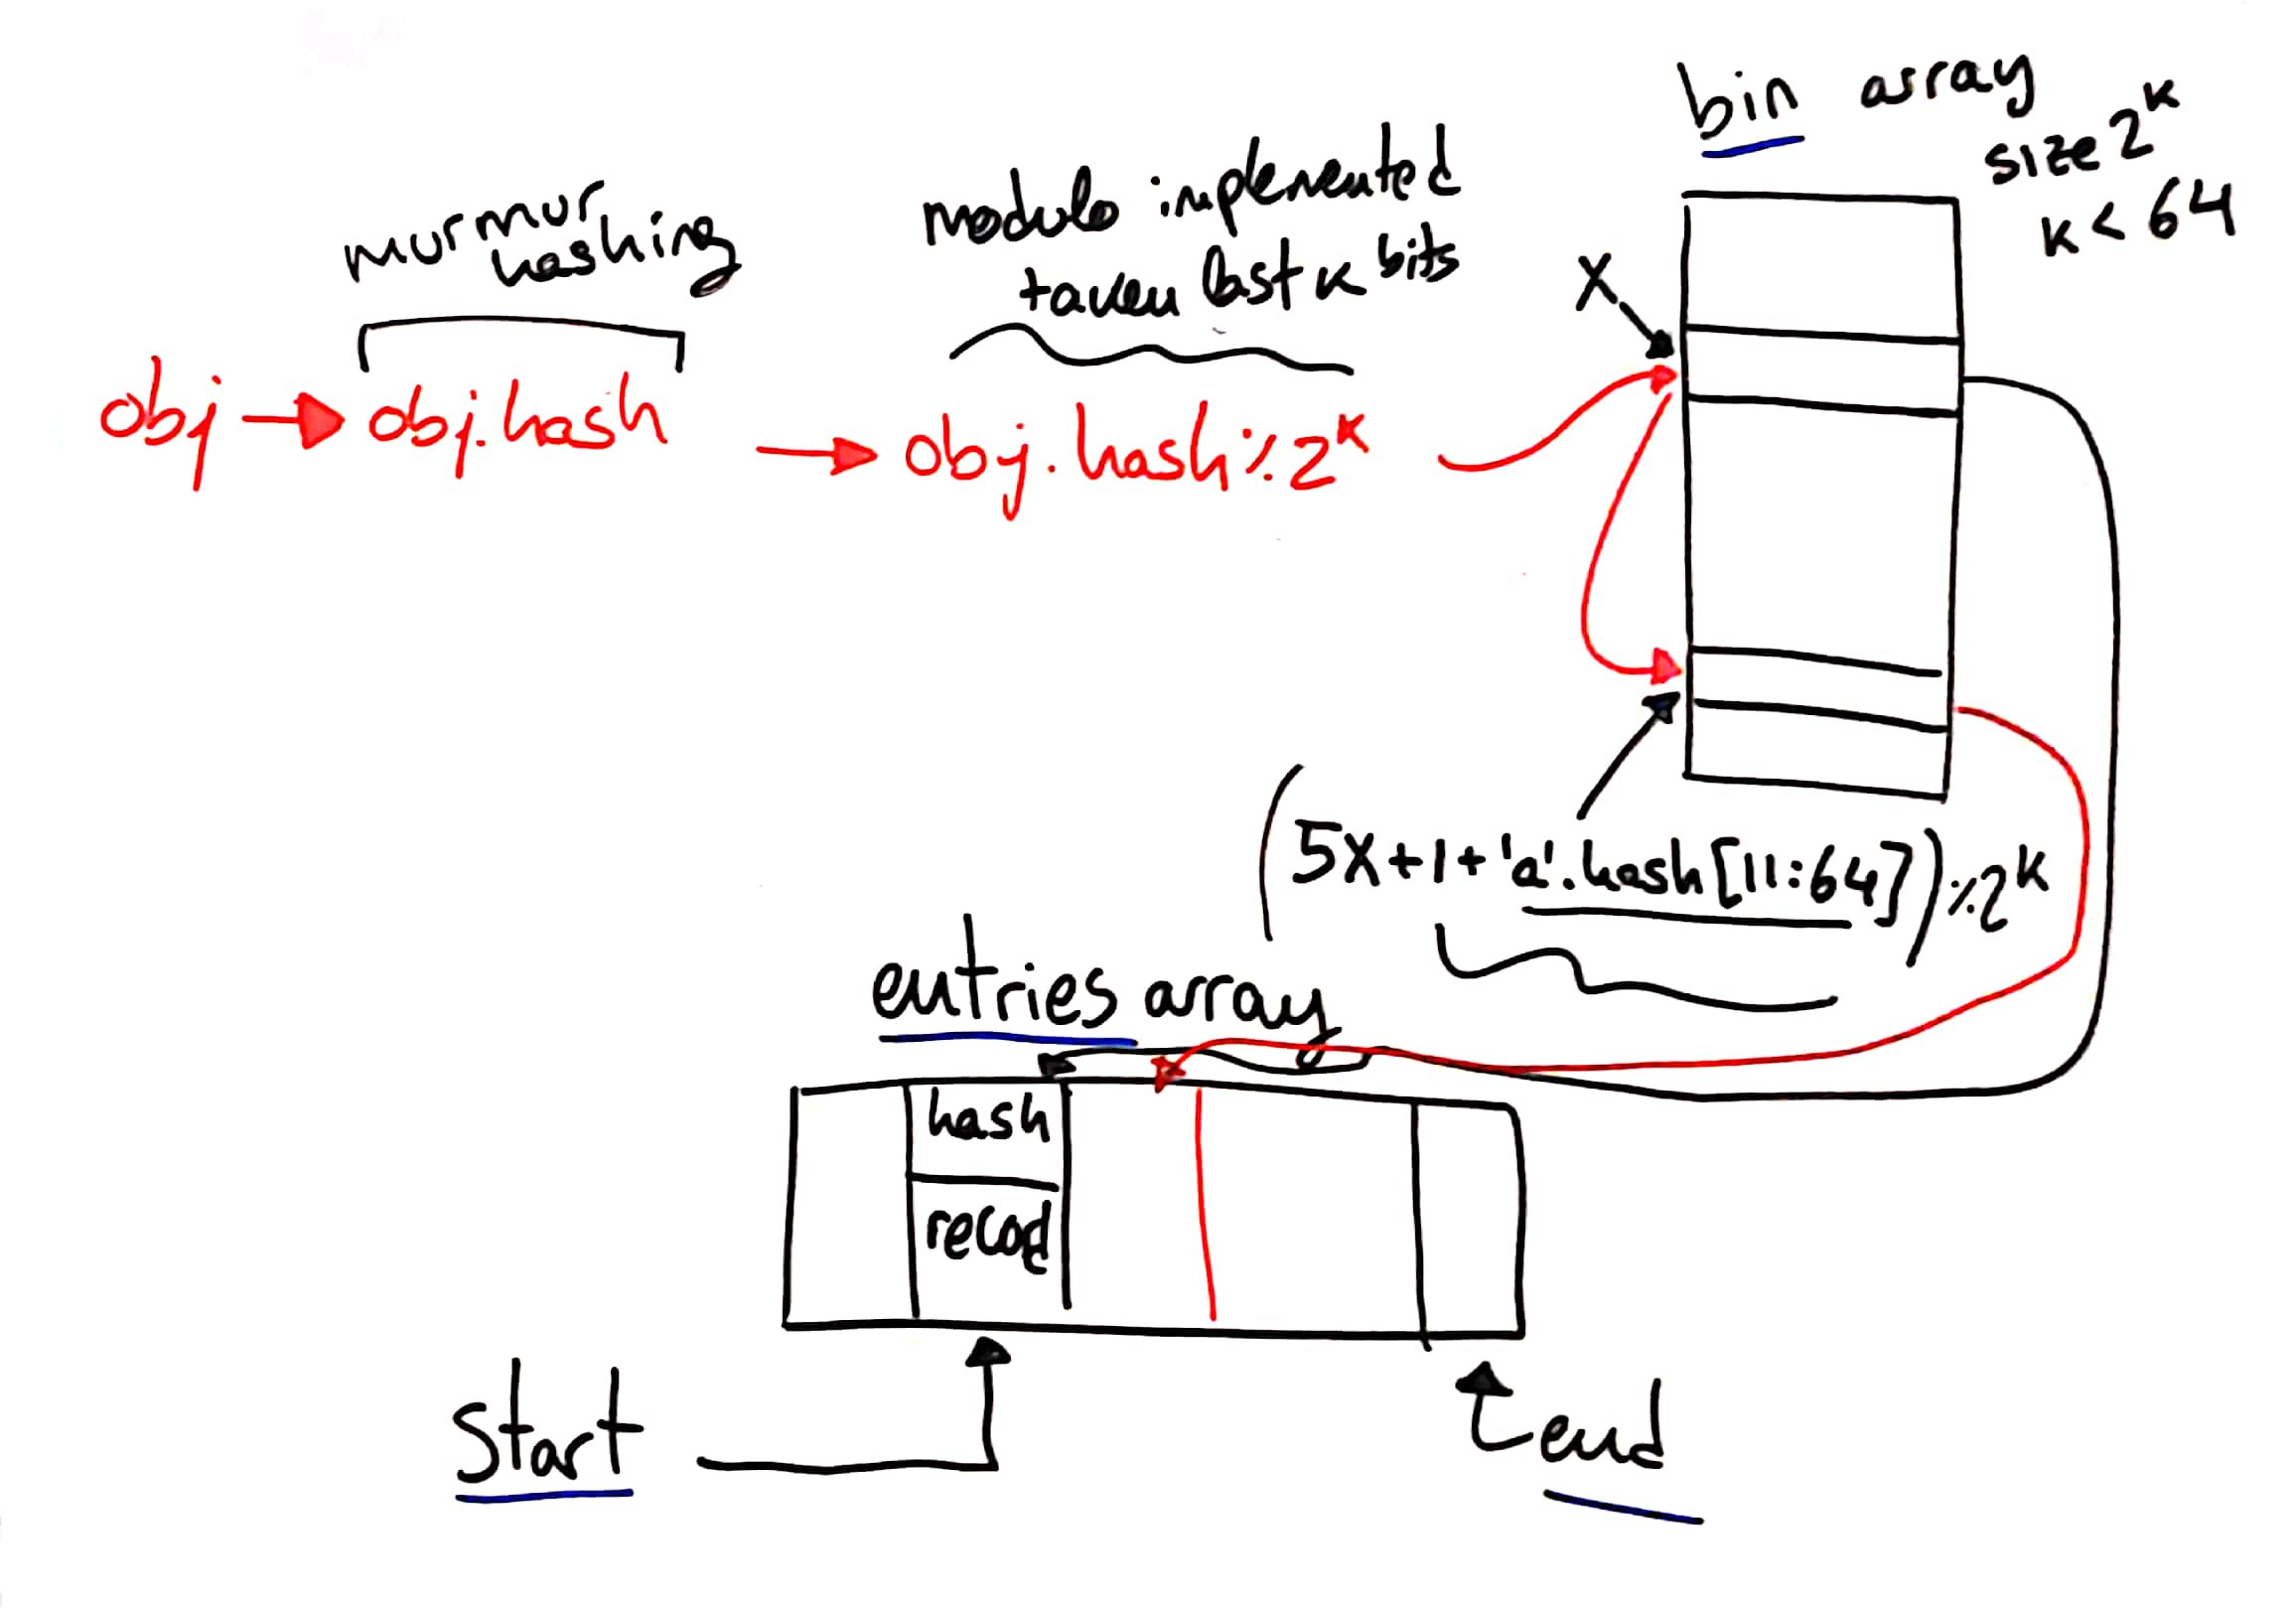
\includegraphics[width=14cm]{hash}}

For more details check \cite{ruby_code} and \cite{ruby_feature12142}.

\subsection{Other important details}

Although not strictly related with the new implementation, it is also worthwhile mentioning that most objects in Ruby are hashed using their C pointer value (unique identifier of the object).
That means that for most object we hash fixed length integers.
This is done using Murmur Hashing.
However, there are some exceptions with objects that are compared by their value: numbers, symbols, arrays and hashes.
For example, two difference instances of the array \lstinline{[1,2]} should have the same hash key.
In the case of arrays and hashes, the code iterates over all elements creating a cumulative hash key.
In the case of strings, the SipHash algorithm is used.
This algorithm is used in the hashtable implementation of many other known software, such as Python, Haskell and systemd.
Note that for Strings we wouldn't be able to use Tabulation Hashing, as a Cryptographic hash function is needed.\\

\label{before}
Another important detail I realized of while working on the project implementation is the fact that the \lstinline{hash} method is not used in the hashing for some classes.
The Ruby documentation \cite{object-hash} claims that the hash value is used along with \lstinline{eql?} by the Hash class to determine if two objects reference the same hash key.
But this is not true for the objects mentioned in the previous paragraph.
Consequently, overriding the \lstinline{hash} method in those classes only changes the returned value of the \lstinline{hash} method, but not the hashing implementation.\\
\url{https://bugs.ruby-lang.org/issues/16850}\\

\section{My implementation}

The C code I wrote can be found in the \href{https://github.com/Ana06/ruby/tree/tabulation_project}{\lstinline{tabulation\_project}} branch of my fork of the Ruby project (\acrshort{mri}) in GitHub.
You can see the changes here:\\
\url{https://github.com/Ana06/ruby/compare/master...Ana06:tabulation_project}\\

\subsection{Quadratic Probing}

Quadratic Probing was implemented in \cite{ruby_code} at the same time than the current implementation and it is still in the current code (although it is disabled and not compiled).
More in detail about how it is implemented, if we call \lstinline{h(x)} to the hash function which maps \lstinline{x} to a position in the hash, then the i-th probe position for \lstinline{x} in the Ruby code is given by the following function:\\
\[h(x,i) = h(x) + \frac{1}{2}i + \frac{1}{2}i^2\]

\vspace{3mm}

This produces the following probe sequence:\\
\[h(x), h(x) + 1, h(x) + 3, h(x) + 6, h(x) + 10, \dots \]

\vspace{2mm}

In this sequence the increase values are triangular numbers, making it efficient to implement.\\

I enabled Quadratic Probing in \commitUrl{\commitQuadratic}{\commitQuadraticShort} and confirmed it is still working.\\

\subsection{Linear Probing}

In \commitUrl{\commitLinear}{\commitLinearShort}, I implemented Linear Probing, which was straightforward by using the already existing code for Quadratic Probing.
More in detail, if we call \lstinline{h(x)} to the hash function which maps \lstinline{x} to a position in the hash, then the i-th probe position for \lstinline{x} is given by the following function:\\
\[h(x,i) = h(x) + i\]

\vspace{2mm}

In other words, if a collision occurs, we try the next hash cell until we find an empty one.\\

\subsection{Tabulation}
\subsubsection{Implementation of Simple, Twisted and Double Tabulation in Ruby}

I implemented Simple, Twisted and Double Tabulation \cite{10.1145/3068772}.
This part was not easy to do in C because of the complexity of the existing code.
Because of that, I started by implemented it in Ruby, overwriting the \lstinline{hash} method.
As I mentioned in \ref{before}, this is not possible for all objects, but it is possible for general classes, the case we are focusing on.
I wrote several methods for different types of Tabulation, which can be found in the following url together with the benchmarking code used:\\
\url{https://github.com/Ana06/ruby-tabulation/blob/master/tabulation_hashing.rb}\\
Below are the times (in seconds) I got executing this code:

\begin{itemize}
\item \textbf{Current master implementation: 29.63}
\item \textbf{Simple tabulation 1: 466.82}\\
64 bits hash by splitting the input in 8 pieces of 1 byte (needing 16KB of randomly filled storage).
This first version of Simple Tabulation uses some readable Ruby methods (such as \lstinline{pack}), which makes it really slow.
The reason why I provided this example is to illustrate that even a small mistake when implementing Tabulation Hashing or when modifying the Ruby Code could modify our results significatively.
\item \textbf{Simple tabulation 2: 154.26}\\
It also implements a 64 bits hash by splitting the input in 8 pieces of 1 byte (needing 16KB of randomly filled storage), but doesn't use slow Ruby methods, making it much faster.
\item \textbf{Simple tabulation 3: 270.35}\\
64 bits hash by splitting the input in 16 pieces of 4 bites.
This version is slower than the previous one, but it has a smaller randomly filled storage of 2KB.
\item \textbf{Twisted tabulation: 185.25}\\
64 bits hash by splitting the input in 8 pieces of 1 byte.
I suspect that the reason why this is slower than the simple tabulation version is that it uses 128 bits integers, which is not a C native type.
Consequently, this is internally represented as two 64 bits integers and some operations are more expensive.
In addition, it needs 32KB of randomly filled storage.
\item \textbf{Double tabulation: 299.4}\\
It implements Double Tabulation by applying twice simple tabulation 2 (with two different randomly filled storages, 32KB in total).
Although Double tabulation is highly independent, it seems that this doesn't make such a different in our case to overcome the extra computational cost.
\end{itemize}

Although it is clear that by overwriting the \lstinline{hash} method in Ruby we can not get even close to the results from the C implementation, we get some interesting results.
First, we need to be especially carefull with making small mistakes when modifying such an important part of a programming language.
Small mistakes could compromise performance.
Second, we get a higher bound on the time that our C implementation should take.
If when implementing Simple Tabulation in C it takes more than 155 seconds, there is something wrong.
I found this really useful when writing the C code, as I had originally written a small typo which made the time bigger than 155 seconds.
If I hadn't known that this time couldn't be correct, I would have thought that Tabulation Hashing doesn't help instead of it being a bug.
Last, we can expect Simple Tabulation to perform better than Twisted and Double Tabulation, also when being implemented in C.
It would be even tricky to write Twisted Tabulation, as there is no gcc support to express an integer constant of 128 bits \cite{gcc128}.
Therefore I focused on implemented Simple Tabulation in C.\\

\subsubsection{Implementation of Simple Tabulation in C}

I implemented Simple Tabulation for the Ruby Code in C in \commitUrl{\commitSimpleTab}{\commitSimpleTabShort}.
As I mentioned before, the part of the code where Simple Tabulation has to be introduced is complicated.
Because of that I implemented it as a proof of concept and not as something that could already be used in production.
The code is not in the correct place and it is only implemented for 64 bits and for the general case (excluding some types such as strings).
But this is enough to prove the potential of Simple Tabulation.\\

The following script benchmarks the insertion of 600000 objects (by hashing their 64 bits ids) in an empty hash 100 times:\\
\url{https://github.com/Ana06/ruby-tabulation/blob/master/benchmark_tabulation.rb}\\
Before starting the benchmarking, it inserts one element in a different hash to ensure that the filling of the random matrix is not benchmarked.
This is needed because, as mentioned before, the code is not in the correct place.
Below are the times (in seconds) I got executing this code for different versions of the Ruby code:\\
\textbf{
\begin{itemize}
\item master (without Simple Tabulation): 29.68
\item master with Linear Probing (without Simple Tabulation): 99.76
\item master with Quadratic Probing (without Simple Tabulation): 29.97
\item master with Simple Tabulation: 15.76
\item master with Linear Probing and Simple Tabulation: 24.23
\item master with Quadratic Probing and Simple Tabulation: 13.73\\
\end{itemize}
}

Note that masters refers to the following Ruby version:\\
\lstinline{ruby 2.8.0dev (2020-05-07T16:22:38Z master 7ded8fd29a) [x86_64-linux]}\\
This is the current Ruby version, which is unreleased and in development.
In fact, I discovered a possible bug while working on the project, which especially affects the master version:
\url{https://bugs.ruby-lang.org/issues/16840}
This means that using an older Ruby version would produce faster results.
I executed the code using 8 x Intel i5-8265U.\\

Even if the code is not in the right place and the calls to some functions I have commented out could slightly modify the results, we can conclude that Quadratic Probing with Tabulation Hashing improves significantly the performance in comparison to the current implementation.
The current approach proved to produce less collisions than quadratic probing (without using Simple Tabulation), although it has worse data locality.
This could have been the case because the given data was not random enough.
Simple Tabulation seems to solve this problem.
In fact, any of the tried hashing algorithms (including the one used currently) perform good with Simple Tabulation, improving the current implementation.
This is a proof that when not having random data, we can not expect that the mathematical properties in which hashing algorithms are based are still verified.
Simple Tabulation helps us to achieve good result even with organized and structure data.
Concretely in this example, we have used classes created in a loop.
If we take a look to a sample of 20 consecutive created classes ids, we can appreciate that this data is not random:

\begin{lstlisting}
11999660
11999680
11999700
11999720
11999740
11999760
11999780
11999800
11999820
11999840
\end{lstlisting}


\section{Conclusion}

The hashing in Ruby (and probably in other programming languages as well) is complicated and involves several techniques and algorithms to ensure its efficiency.
This and the complexity of the code were the biggest challenges I faced during the project.
But it was also an opportunity to learn a wide range of different things, especially from the changes in \cite{ruby_code}.\\

It was also astonishing that being Simple Tabulation such a simple approach can provide such good guarantees.
It was rewarding to not only read about it and its theoretical foundations, but to prove how it can improve the performance in a real world project as Ruby.
I have opened an issue in Ruby presenting the results of the project and the written code:\\
\url{https://bugs.ruby-lang.org/issues/16851}


\printglossary[type=\acronymtype]

\bibliographystyle{plain}
\bibliography{project}

\end{document}

